%%% template.tex
%%%
%%% This LaTeX source document can be used as the basis for your technical
%%% paper or abstract.

%%% The parameter to the ``documentclass'' command is very important.
%%% - use ``review'' for content submitted for review.
%%% - use ``preprint'' for accepted content you are making available.
%%% - use ``tog'' for technical papers accepted to the TOG journal and
%%%   for presentation at the SIGGRAPH or SIGGRAPH Asia conference.
%%% - use ``conference'' for final content accepted to a sponsored event
%%%   (hint: If you don't know, you should use ``conference.'')

\documentclass[tog]{acmsiggraph}

%%% Make the ``BibTeX'' word pretty...

\def\BibTeX{{\rm B\kern-.05em{\sc i\kern-.025em b}\kern-.08em
    T\kern-.1667em\lower.7ex\hbox{E}\kern-.125emX}}

%%% Used by the ``review'' variation; the online ID will be printed on 
%%% every page of the content.

\TOGonlineid{45678}

%%% Used by the ``preprint'' variation.

\TOGvolume{0}
\TOGnumber{0}

\title{Real-Time tearing and fracturing}

\author{Myriam Beauvais\thanks{e-mail:myriam.beauvais@mail.mcgill.ca} \\ ID 260760034 \\COMP-559, Fundamentals of Computer Animation}
\pdfauthor{Stephen N. Spencer}

\keywords{tearing, fracturing, deformation, animation}

\begin{document}

%%% This is the ``teaser'' command, which puts an figure, centered, below 
%%% the title and author information, and above the body of the content.

 \teaser{
   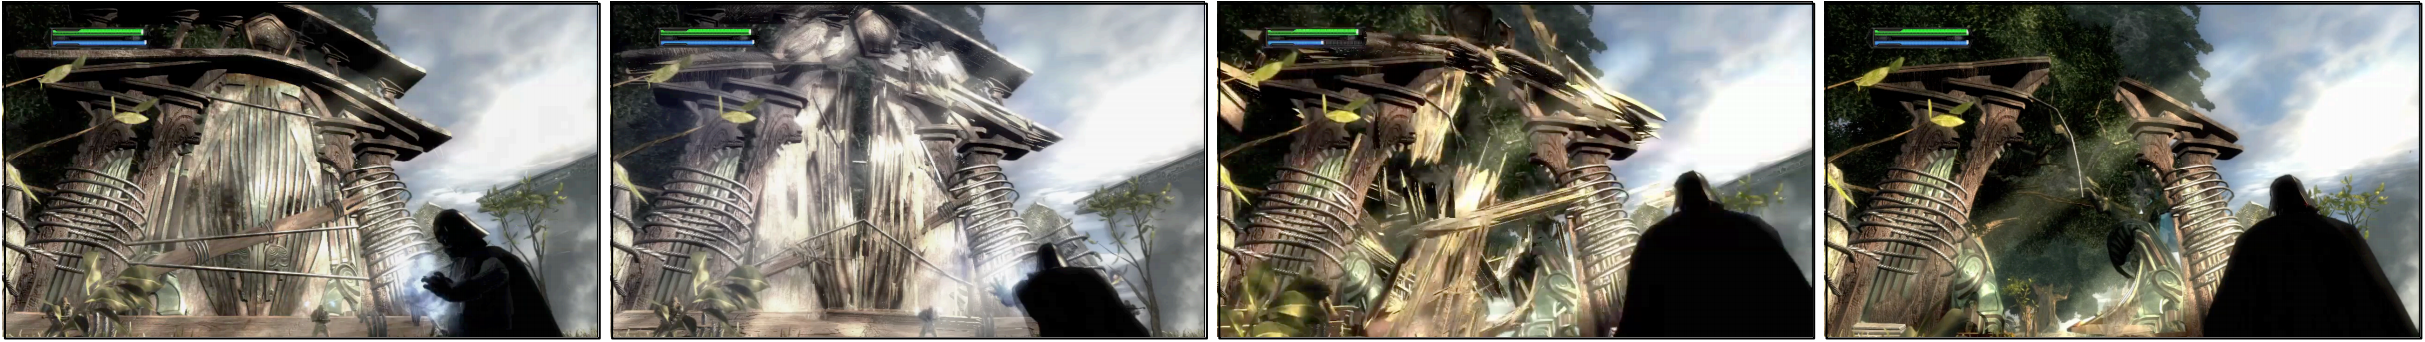
\includegraphics[height=0.98in]{images/Teaser}
   \caption{Star Wars: The Force Unleashed game content and screenshots courtesy of LucasArts, a division of Lucasfilm Entertainment Company Ltd. \copyright 2009 Lucasfilm Entertainment Company Ltd. or
Lucasfilm Ltd. All rights reserved. Image taken from Parker and O'Brien, 2009}
 }

\maketitle

\copyrightspace

\section{Introduction}
A lot of different objects, when under some persistent and or increasing forces, will end up getting distorted and breaking apart. Because virtual objects are often put in such situations in video games, movies or simulations, addressing this topic is very pertinent and interesting in order to recreate realistic sequences.  

The project proposed is the implementation of an interactive application allowing for deformation, tearing and fracturing of meshes in real-time, according to the method described in \cite{Parker:2009:RTD}. Optionally (in function of the advancement and progress rate), to improve the deformation of a mesh the technique described by \cite{Rivers:2007:FFL} will also be implemented. 

\section{Methodology}
\begin{list}
\item Implementation of a basic fps camera, and of a picker (modified for using forces)
\item Creation of the scene : 
	\begin{list}
	\item Create particles as gameobjects with sphere primitives, having bound the Rigid Body script as component to enable PhysX (Unity's physics engine) calculations of collisions.
	\item bind particles with joints. Used HingeJoints (describe various tests done). Add reflexion about use of spring.cs (and actually use it if have time to)
	\item Create a mesh having vertices at the particles' position. 
	\item reupdate the mesh according to the particles new positions (indices stay the same
	\item Although the scene is in 3D, all calculations and implementations take into account that we are only dealing with planes.  
	\end{list}
\item Fracturing...

\end{list}


\subsection{Additional concepts and tools needed}

\begin{tabular}{|c|c|}
\hline
Element needed & Solution\\
\hline
\hline
3D Viewer & Unity project\\
Interface & Unity's UI tool \\
Linearized Backward Euler Integrator & Self-Implemented\\
Collision Detection & Unity's physic engine\\
\hline
\end{tabular}


%%\section{Figures and Tables and Captions}

%%Figures and tables can span one or both columns. Captions for figures
%%should be centered underneath the figure. Captions for tables should
%%be centered above the table.

%%\begin{table}[ht]
%%  \centering
%%  \caption{A simple table.}
%%  \begin{tabular}{|r|l|}
%%    \hline
%%    7C0 & hexadecimal \\
%%    3700 & octal \\ \cline{2-2}
%%    11111000000 & binary \\
%%    \hline \hline
%%    1984 & decimal \\
%%    \hline
%%  \end{tabular}
%%\end{table}
  
%%Please use 9-point bold serif type for the caption title, and 9-point
%%serif type for the caption text (both on 10-point line spacing).

%\section{Citations and References}
%
%\subsection{Citations}
%
%The SIGGRAPH citation format is the ``author year''
%format~\cite{Pellacini:2005:LAH}. The year is separated from the
%author by a single space~\cite{yee:2000:ssa}. Two authors are
%separated by the word ``and''~\cite{parke:1996:CFA}. More than two
%authors are represented by the primary author and ``et al.''~\cite{levoy:2000:TDM}.
%
%Multiple citations at a single point in the content are separated by
%semicolons~\cite{levoy:2000:TDM,sako:2001:SSB}.
%
%When the last name of the cited author is part of the text, it may be
%omitted from the citation: ``\ldots as shown in Fedkiw et
%al.~\shortcite{fedkiw:2001:VSO}, the coefficient remains\ldots''
%
%\subsection{References}
%
%The reference list, or bibliography, must be unnumbered, alphabetized
%by the primary author's last name, followed by the year of publication
%and other identifying information (article title, journal title,
%volume, number, etc.). Author names are arranged as ``last name,
%initials.'' The page number, if any, is the last piece of information
%in the reference.
%
%The first line of each entry in the bibliography has no
%indentation. The second successive lines has a 2em
%indentation. 
%
%Please use 9-point serif type, with 10-point line spacing, for each
%entry in the bibliography, with a single blank line between each
%entry. 
%
%Journal, book, thesis, and conference proceedings titles are set in an
%italic serif type. {\sc Author names should be typeset in a ``Small
%Caps'' typeface.}
%
%\section{Third-Party Material}
%
%If you are using third-party material in your content - that is,
%material which you or your co-authors did not create - you need to
%clearly identify it as such in the material itself or in the 
%content's caption, as shown in Figure~\ref{fig:ferrari}.
%
%\begin{figure}[ht]
%  \centering
%  \includegraphics[width=3.0in]{images/ferrari_laferrari}
%  \caption{Ferrari LaFerrari. Image courtesy Flickr user ``gfreeman23.''}
%  \label{fig:ferrari}
%\end{figure}
%
%ACM's policy on third-party material can be found at the following link:
%
%{\small\url{http://www.acm.org/publications/third-party-material}}


\bibliographystyle{acmsiggraph}
\nocite{*}
\bibliography{template}
\end{document}
